% requires the hyperref package
% also requires graphicx

\section{The Control System}

This section describes the embedded control system and user interaction.
The latest system software and documentation can always be found on github at \url{https://github.com/hedj/fusion/}.

Flowcharts in this section use the visual language from the DRAKON project. See \url{http://drakon-editor.sourceforge.net/language.html} for details.

\begin{figure}
  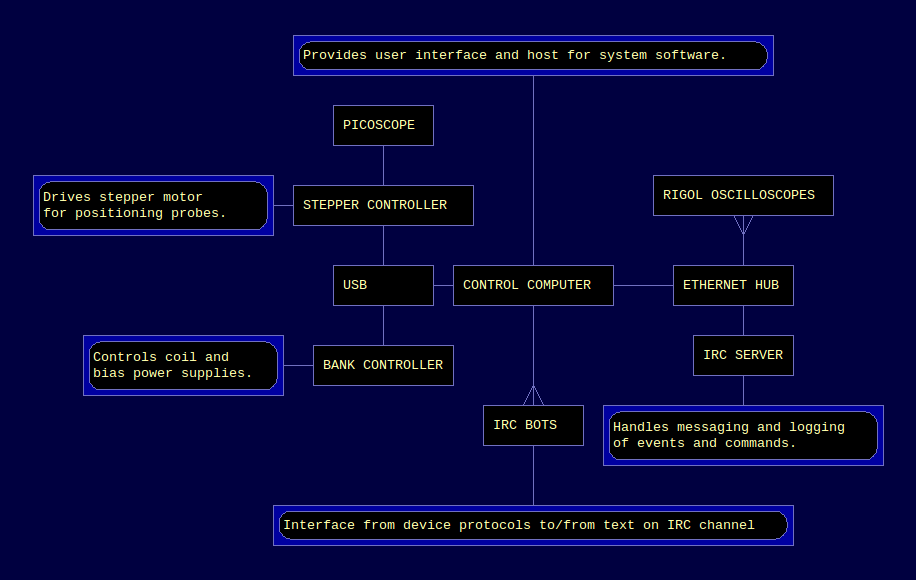
\includegraphics[width=400px]{system_structure.png}
\caption{\label{fig:system} Overall system design}
\end{figure}

\subsection{The Bank Controller}

The bank controller is a \href{http://controllino.biz/product/controllino-mega/}{Controllino Mega}; an
Arduino-based programmable-logic controller. The bank controller is in charge of the following functions:
\begin{itemize}
  \item{Capacitor-bank and HV pulse generation}
  \item{HV voltage control}
  \item{Capacitor bank charge control}
  \item{Audible alert before pulse}
\end{itemize}

The top-level flow of the bank controller is shown in Fig.~\ref{fig:toplevelbank}.

\begin{figure}
  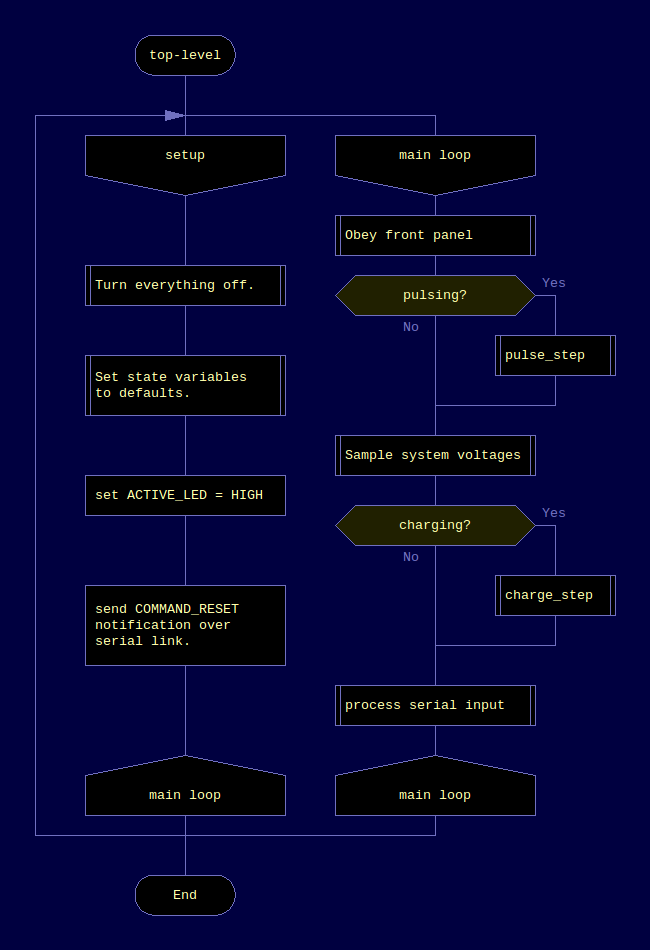
\includegraphics[width=400px]{top_level.png}
\caption{\label{fig:toplevelbank} Top-level flow of the bank controller}
\end{figure}

The serial protocol used is nonstandard; a definition can be found at \url{https://github.com/hedj/nslc}.  It is designed to facilitate debugging using a serial terminal; nslc is a simple frame-based protocol using line-feeds as end-of-frame markers and whitespace for escape. It is also checksummed for reliability. The particular checksum is only 8 bits in size, and is optimised for speed of implementation.

The most important thing to emphasise is that the controller is implemented as a tight loop reacting to the change in time. There are no blocking wait statements; in this way we ensure that input can continue to be received from the front panel switches or serial as the process runs. This allows the safe abort of the system regardless of its state, which is rather important.

The two operations which consume a reasonable amount of time and are thus implemented as conditional actions in the inner loop are pulsing and charging, respectively Figs.~\ref{fig:pulse_step}~and~\ref{fig:charge_step}.

\begin{figure}
  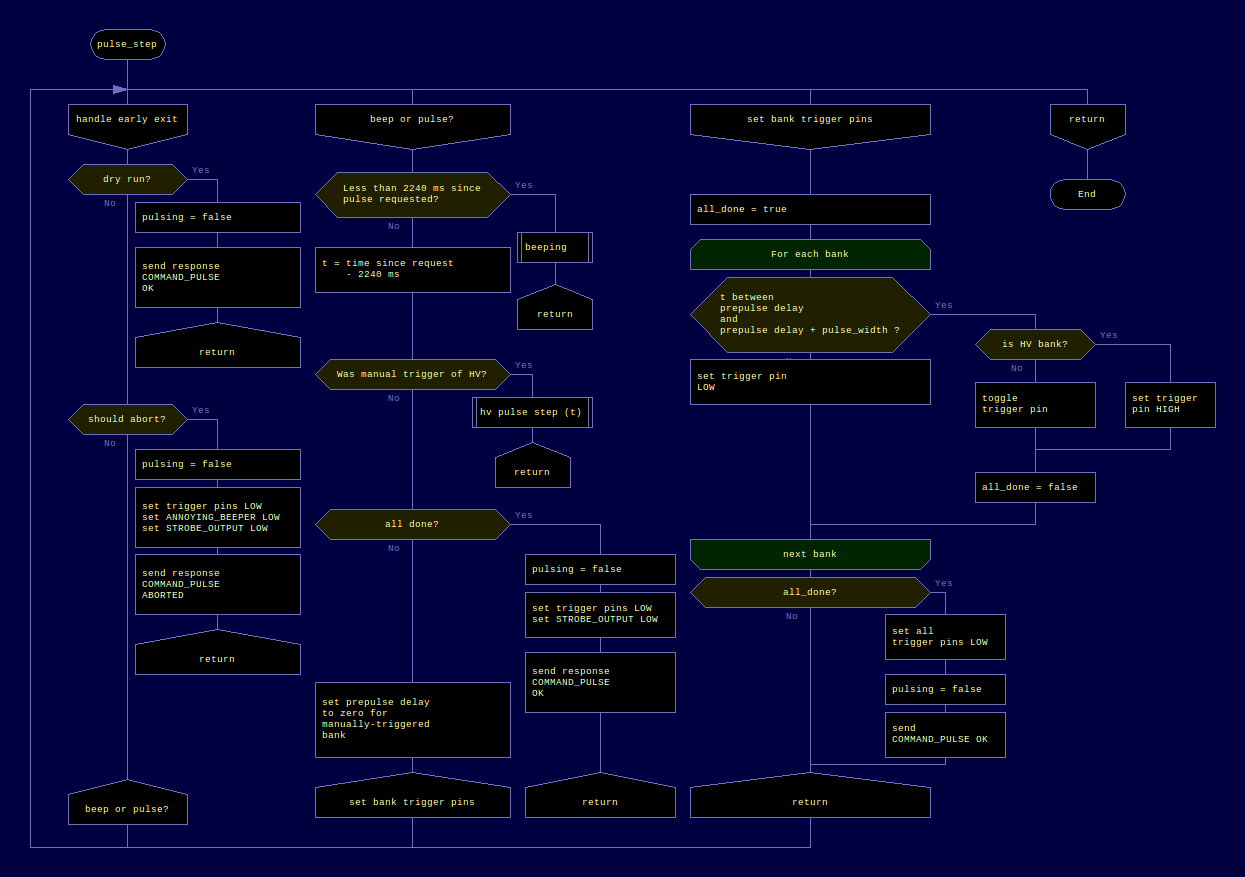
\includegraphics[width=400px]{pulse_step.png}
\caption{\label{fig:pulse_step} Pulse Step processing}
\end{figure}

\begin{figure}
  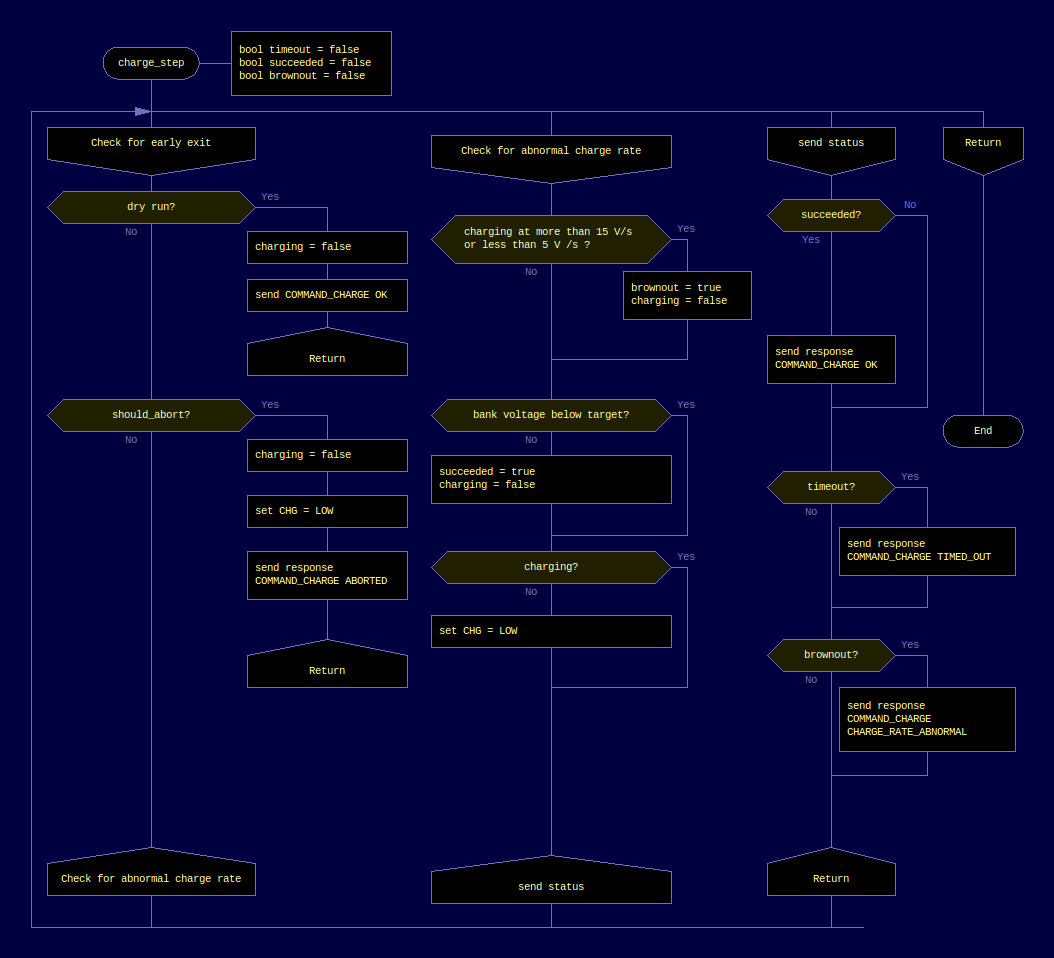
\includegraphics[width=400px]{charge_step.png}
\caption{\label{fig:charge_step} Charging step logic}
\end{figure}


\subsection{The Stepper Controller}
\subsection{The IRC Server}
\subsection{The Agents}
\subsection{Using the System}
